% CVPR 2025 Paper Template; see https://github.com/cvpr-org/author-kit

\documentclass[10pt,twocolumn,letterpaper]{article}

%%%%%%%%% PAPER TYPE  - PLEASE UPDATE FOR FINAL VERSION
% \usepackage{cvpr}              % To produce the CAMERA-READY version
\usepackage[review]{cvpr}      % To produce the REVIEW version
% \usepackage[pagenumbers]{cvpr} % To force page numbers, e.g. for an arXiv version

\usepackage{amsmath} % assumes amsmath package installed
\usepackage{verbatim} % 块注释
% \begin{comment} 
	%	... (需要被注释段落)
	% \end{comment}

% Import additional packages in the preamble file, before hyperref
%
% --- inline annotations
%
\newcommand{\red}[1]{{\color{red}#1}}
\newcommand{\todo}[1]{{\color{red}#1}}
\newcommand{\TODO}[1]{\textbf{\color{red}[TODO: #1]}}
% --- disable by uncommenting  
% \renewcommand{\TODO}[1]{}
% \renewcommand{\todo}[1]{#1}



% It is strongly recommended to use hyperref, especially for the review version.
% hyperref with option pagebackref eases the reviewers' job.
% Please disable hyperref *only* if you encounter grave issues, 
% e.g. with the file validation for the camera-ready version.
%
% If you comment hyperref and then uncomment it, you should delete *.aux before re-running LaTeX.
% (Or just hit 'q' on the first LaTeX run, let it finish, and you should be clear).
\definecolor{cvprblue}{rgb}{0.21,0.49,0.74}
\usepackage[pagebackref,breaklinks,colorlinks,allcolors=cvprblue]{hyperref}

%%%%%%%%% PAPER ID  - PLEASE UPDATE
\def\paperID{*****} % *** Enter the Paper ID here
\def\confName{CVPR}
\def\confYear{2025}

%%%%%%%%% TITLE - PLEASE UPDATE
% \title{\LaTeX\ Author Guidelines for \confName~Proceedings}
\title{A Brain-Inspired Perception-Decision Driving Model \\Based on Neural Pathway Anatomical Alignment}

%%%%%%%%% AUTHORS - PLEASE UPDATE
\author{First Author\\
Institution1\\
Institution1 address\\
{\tt\small firstauthor@i1.org}
% For a paper whose authors are all at the same institution,
% omit the following lines up until the closing ``}''.
% Additional authors and addresses can be added with ``\and'',
% just like the second author.
% To save space, use either the email address or home page, not both
\and
Second Author\\
Institution2\\
First line of institution2 address\\
{\tt\small secondauthor@i2.org}
}

\begin{document}
\maketitle
\begin{abstract}
In the realm of autonomous driving, conventional approaches for vehicle perception and decision-making primarily rely on sensor input and rule-based algorithms. 
However, these methodologies often suffer from lack of interpretability and robustness, particularly in intricate traffic scenarios. 
To tackle this challenge, we propose a novel brain-inspired driving (BID) framework. 
Diverging from traditional methods, our approach harnesses brain-inspired perception technology to achieve more efficient and robust environmental perception. 
Additionally, it employs brain-inspired decision-making techniques to facilitate intelligent decision-making. 
The experimental results show that the performance has been significantly improved across various autonomous driving tasks and achieved the end-to-end autopilot successfully. 
This contribution not only advances interpretability and robustness but also offers fancy insights and methodologies for further advancing autonomous driving technology.
\end{abstract}
    
\section{Introduction}
\label{sec:intro}
\hspace{1pc}Autonomous driving \cite{urmson2008autonomous} is an advanced technology that intelligent vehicles perceive road environments through onboard sensor systems, autonomously plan driving routes, and control vehicles to reach predetermined destinations. 
Its technical system generally includes three major parts: environmental perception, decision planning, and vehicle control~\cite{amini2020learning, montemerlo2008junior}, involving multiple research fields such as computer science, mathematics, mechanical engineering, control science, and psychology~\cite{chen2015deepdriving}.


However, the current autonomous driving systems still suffer from insufficient interpretability due to the existence of ``black box" nature of deep learning models \cite{7979332}, greatly limiting the credibility and widespread application of various perception and decision-making methods in practical engineering. 
Even though the use of generative adversarial networks (GANs) \cite{zugner2020adversarial} to generate explanatory data related to decision-making has been attempted, the quality of such data is often substandard, and the training process is quite challenging. 
Furthermore, modern urban traffic conditions are characterized by high dynamics and strong uncertainty. 
When the environment is complex, the autonomous driving system may experience performance degradation. 
Therefore, to overcome the limitations of existing methods, there is a need to design more interpretable and robust autonomous driving systems, thereby ensuring the safety of vehicle operation.
\begin{figure}[t]
	\centering
	%\fbox{\rule{0pt}{2in} \rule{0.9\linewidth}{0pt}}
	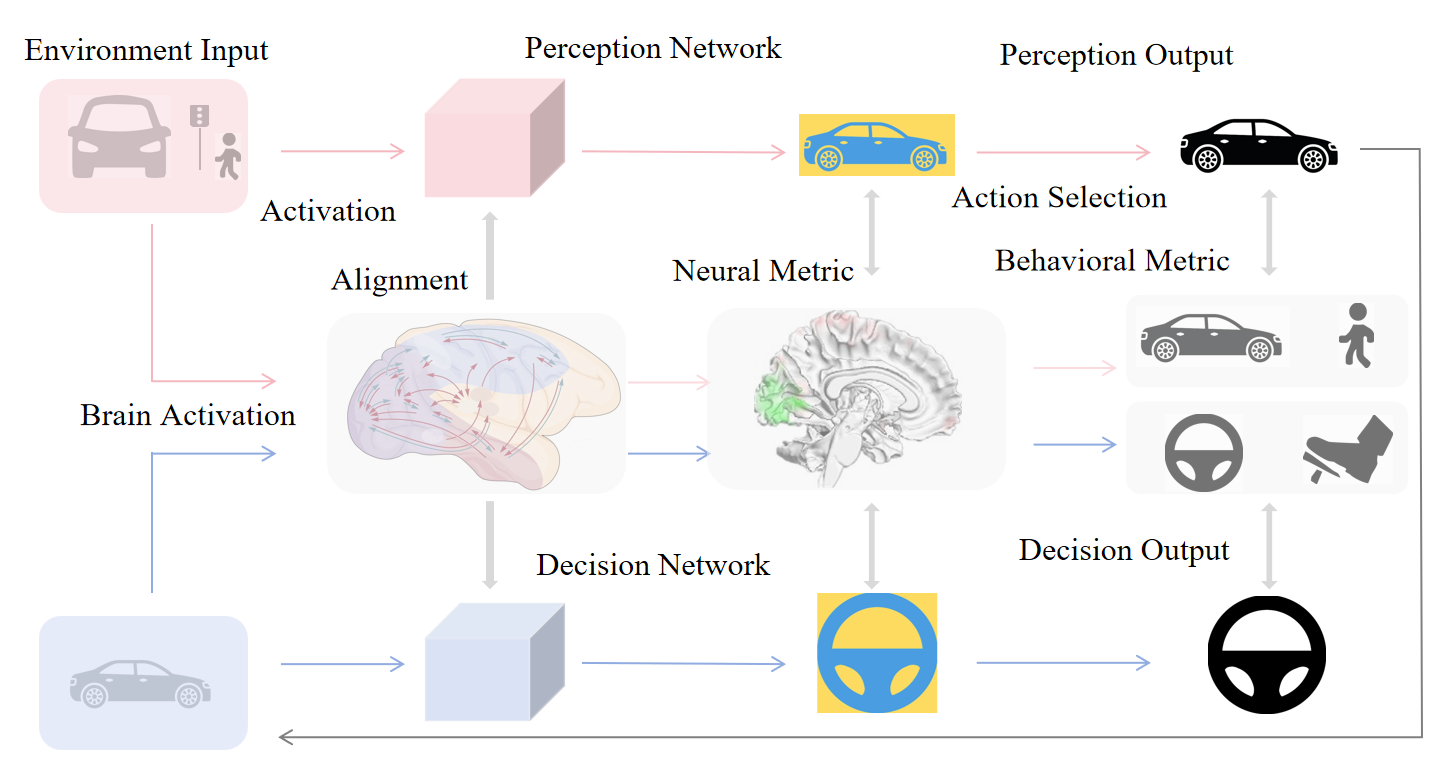
\includegraphics[width=0.95\linewidth]{fig/brain_inspired.pdf}
	\caption{Perception-Decision Network Diagram Based on Neural Pathway Anatomical Alignment}
	\label{fig:fig1}
\end{figure}

In this work, we propose a novel BID framework inspired by brain perception and decision-making. 
Unlike previous methods, our reinforcement learning expert does not rely on manually formulated rules and demonstrates strong interpretability and robustness. 
Our work involves constructing a brain-inspired perception network for extracting environmental features of the target vehicle and a brain-inspired decision-making network for generating driving decisions for the target vehicle, in order to train the reinforcement learning expert~\cite{kahn2021land}. 
Its structure is as shown in Fig.~\ref{fig:fig1}. 
Specifically, the brain-inspired perception network consists of a visual perception module~\cite{al2018brain}, a motion perception module, and a multimodal perception module~\cite{yu2023brain}. 
The brain-inspired decision-making network comprises a decision generation module~\cite{schirner2023learning} and a decision evaluation module. 
Driving decisions encompass multiple driving actions of the target vehicle, and the BID agent directly imitates expert behavior. 
Overall, our main contribution lies in proposing a novel brain-inspired perception model and a brain-inspired decision-making model for autonomous driving, aiming to achieve a more robust and interpretable autonomous driving system.






\section{Related Work}

\subsection{Brain-Inspired Perception}
\hspace{1pc}The human visual cortex possesses remarkable environmental perception capabilities, serving as a crucial component of the central nervous system and responsible for transforming visual signals into comprehensible information \cite{9134376}. 
Traditional visual encoding models are limited by the use of either handcrafted or deep learning features merely, despite their individual advantages\cite{kubilius2019brain}. 
To integrate the two, Cui et al. \cite{8574054} proposed the GaborNet-VE model, which combines Gabor features with deep learning to form an efficient visual encoding framework. 
However, this model requires significant parameter adjustments across different tasks, and the interpretability of its deep learning component remains inadequate\cite{liao2021statistical}. 
In contrast, our proposed BID model demonstrates outstanding performance in revealing decision-making mechanisms and exhibiting strong generalization capabilities.

\subsection{Brain-Inspired Decision}
\hspace{1pc}In practical environments, agents often need to handle continuous state spaces, while traditional reinforcement learning models, such as Q learning methods, are more fit to discrete states\cite{xi2020automatic}. 
To address this issue, Zhao et al. \cite{zhao2018brain} proposed the prefrontal cortex and basal ganglia method, which subdivides continuous states and utilizes a continuous function to capture temporal reward. 
However, the design of continuous reward functions remains a challenge. 
In non-Gaussian and nonlinear environments, traditional methods struggle to cope with their nonlinear and non-Gaussian characteristics\cite{naghshvarianjahromi2020natural}. 
Inspired by human decision-making in brain, some researchers~\cite{dai2013dynamic} designed an autonomous computation layer accroding to a cognitive dynamic system (CDS), providing agents in NGNLE with stronger decision-making capabilities. 
Although these methods attempt to mimic the decision-making process of the human brain, structural differences lead to a lack of transparency in their processes. 
Therefore, it is crucial to construct network models that align with the anatomical structure of human brain.



\section{Method}

BID is trained by imitation learning, which we formalized as follows.
Expert demonstrator (drivers) produce an action $a_i$ (ego-vehicle maneuver) when encountering an observation $O_i$, (sensor data, signals) given the expert policy $\pi^{ \star } (O_i)$ (driving skills, attitude, etc.).
The basic idea behind imitation is to train an agent (here BID) that mimics an expert by using these observation.


Prior to training an agent, we need to collect a dataset comprised of observation/action pairs $P= \{ (o_i, a_i) \}_{i=1} ^N $ generated by the expert.
This dataset is in turn used to train a policy $\pi_\theta (o_i)$ which approximateds the expert policy.
The general imitation learning objective is the 
\begin{equation}
	argmin E_{(o_i, a_i) ~ P} [P(\pi_\theta (o_i), a_i )].
\end{equation}

\begin{figure*}[t]
	\centering
	%\fbox{\rule{0pt}{2in} \rule{0.9\linewidth}{0pt}}
	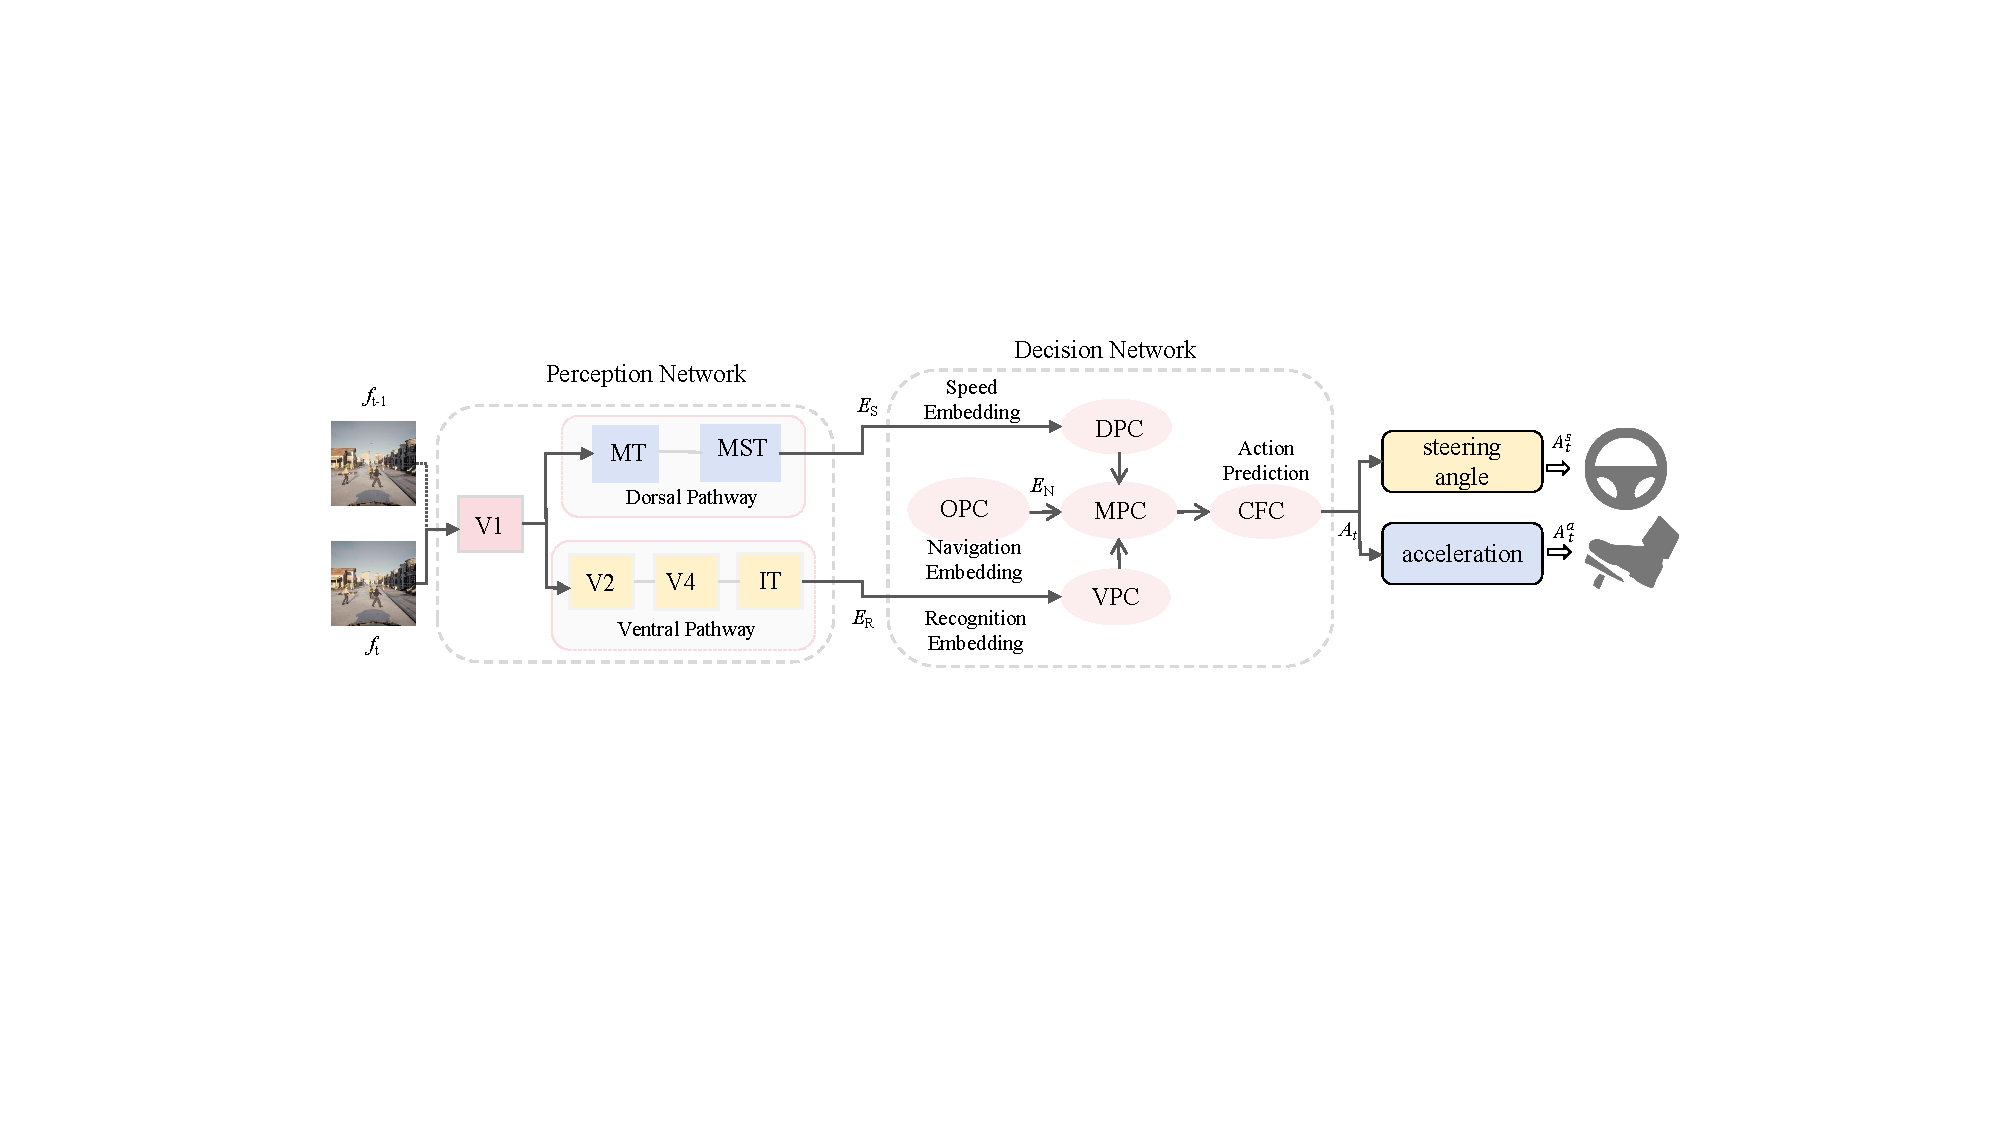
\includegraphics[width=\linewidth]{fig/net}
	\caption{Network architecture of the BID agent:
	our model is mainly comprised of two parts: perception and decision network.
	Perception network include dorsal and ventral pathway to understand their surroundings.
	Decision network include five modules: medial prefrontal cortex (VPC), orbital prefrontal cortex (OPC), caudal prefrontal crotex (CPC), dorsal prefrontal cortex (DPC), ventral prefrontal cortex (VPC).
	Specifically, the input observation consists of RGB image $X_t$.
	The output is action $a_t$, which is directly applied to maneuver to ego-vehicle.
	Since $a_t$ consists of the ego-vehicle's steering angle and acceleration, BID is a vision-based vision-based pure end-to-end AD model.
	Note that these action components are automatically read and associated with the captured images during data collection.
	}
	\label{fig:fig2}
\end{figure*}
\subsection{Neural Aligned Roach}
\hspace{1pc}Drawing inspiration from the brain's exceptional mechanisms in perception and decision-making, we have seamlessly integrated the intricate methods of information processing by brain neurons into an autonomous driving system, aiming to significantly enhance the system's interpretability and robustness. As depicted in Fig. \ref{fig:fig2}, our brain-inspired perception network initially captures precise input data from the surrounding environment, encompassing crucial traffic elements such as roads, vehicles, pedestrians, and traffic signals. Subsequently, this data undergoes meticulous processing through a series of deep convolutional neural networks and recurrent networks, along with the utilization of deep neural network activation functions. This processing mimics the handling of external information by various pathways in the brain's visual cortex. Initially, the primary visual cortex (V1) performs initial processing of visual information, extracting salient features. These features are then relayed to the dorsal visual pathway, where the MT/MST (Middle Temporal and Middle Superior Temporal Areas) encode motion features, specializing in the processing of information related to spatial location and movement. Concurrently, the ventral pathway receives these features, and the IT (Inferior Temporal Cortex) encodes target category information, facilitating object recognition. After this series of processing, our network is able to effectively extract and output multi-dimensional features of the current environment, including the appearance features of objects, motion trajectory features, and the fusion of multi-modal information.

These features are then efficiently transmitted to a brain-inspired decision-making network, undergoing further processing through convolutional and recurrent networks, as well as optimization via deep neural network activation functions. This simulates the processing of sensory outcomes by various regions of the prefrontal cortex in the brain. Among them, the OFC (Orbitofrontal Cortex) plays a vital role in setting future action goals, assisting us in clarifying and locking onto the desired objectives. The MPC ( Medial Prefrontal Cortex) plays a crucial role in making choices based on prior behavioral outcomes, ensuring that our behavior is optimized based on experience. The DPC (Dorsal Prefrontal Cortex) excels at generating goals based on sequences, temporal and spatial environments, providing clear directions and guidance for our actions. The VPC (Ventral Prefrontal Cortex) generates goals based on visual and auditory cues, enabling us to respond quickly and adapt to changes in the external environment.  Meanwhile, the CPC (Caudal Prefrontal Cortex) plays an indispensable role in searching, identifying, or locating specific targets, ensuring that we can accurately locate and focus on the targets.  These regions collaborate and participate in decision-making, generating a highly integrated latent feature vector that precisely encapsulates the critical information required for decision-making. Finally, this latent feature vector is mapped through a carefully designed hidden layer, outputting precise and reliable decision-making information such as driving actions, value function estimates, and speed control.

\textbf{\textsf{Reward Function.}} The BID network aims to mimic the superior information processing capabilities of the human brain by meticulously comparing brain activation patterns with network activation patterns. 
It iteratively updates its network parameters to align network decisions more closely with the actual decision-making mechanisms of the human brain, thereby enhancing the performance and accuracy of the network. 
The specific methodology for updating the network is outlined as follows:
\begin{align}
	\theta_{k+1} & = \arg \max _{\theta} \underset{\tau \sim \pi_{\theta_{k}}}{\mathrm{E}}\left[\mathcal{L}_{\mathrm{ppo}}+\mathcal{L}_{\text {pre }}+\lambda_{\text {e }} \cdot \mathcal{L}_{\text {exp }}\right]
\end{align}

Simulating the approach the brain acquires rewards, aiming to maximize reward-seeking behavior. We train the decision network using Proximal Policy Optimization (PPO) \cite{schulman2017proximal} with clipping. $\mathcal{L}_{\text {ppo }}$ serves as the dopamine reward signal. It is understood that when the brain predicts an upcoming reward, the dopamine system becomes active, generating a reward signal. This signal can be seen as feedback from the brain regarding specific behaviors or situations, informing the brain whether the behavior or situation is positive or worth pursuing. $\mathcal{L}_{\text {pre }}$ represents the prediction error of brain reward. This error arises when there is a deviation between the actual reward and the expected reward. In this context, the reward prediction error functions as a penalty term. Specifically, if the actual reward ($a_{r}$) falls below the expected reward ($p_{r}$), the reward prediction error is negative.Additionally, $\mathcal{L}_{\text {exp }}$ encapsulates the exploration of new actions or strategies during the learning process to obtain more rewards, with $\lambda$ serving as their weight parameter.

Considering both the certainty of the policy (via the entropy regularization term) and the accuracy of reward prediction (via the reward prediction error term), this guides the model to learn more accurate reward predictions, thereby enhancing its performance in reinforcement learning tasks. Specifically, The constant (C) serves to adjust the numerical range or optimization scale of the entropy.
\begin{align}
	\mathcal{L}_{\text{pre}} & = -\lambda_{\text {p }} \cdot [\mathrm{H}\left(\pi_{\theta}\left(\cdot \mid \mathbf{i}_{\mathrm{NR}}, \mathbf{m}_{\mathrm{NR}}\right)\right) - (a_{r} - p_{r})^{2}]
\end{align}
\begin{align}
	\mathrm{H}\left(\pi_{\theta}\right) & = -\mathrm{KL}\left(\pi_{\theta} \| \mathcal{U}(-1,1)\right)+C
\end{align}

Regularizing the whole trajectory to better utilize previous experience and improve the efficiency and stability of learning.
\begin{align}
    \mathcal{L}_{\text {exp }}=\sum_{k=1}^{T} f(k) \cdot \mathrm{KL}\left(\pi_{\theta}\left(\cdot \mid \mathbf{i}_{\mathrm{NR}, k}, \mathbf{m}_{\mathrm{NR}, k}\right) \| p_{z}\right)
\end{align}

\textbf{\textsf{Training.}} The vehicle solely utilizes a single camera sensor to capture raw data of its surrounding environment. At the input stage, it receives a Bird's Eye View (BEV) semantic segmentation image, denoted as $\mathbf{i}_{\mathrm{NR}}$, along with a measurement vector, $\mathbf{m}_{\mathrm{NR}}$, from its own roach system. After acquiring these input data, the BID network is activated to simulate the brain's visual processing. When predicting or receiving rewards, simulated dopamine neurons are activated, releasing dopamine to strengthen memories and behaviors associated with the rewards, increasing the likelihood of repeating these behaviors. During the learning process, there is often a mismatch between expected and actual rewards. When actual rewards exceed expectations, a positive prediction error occurs, further promoting the release of dopamine and thus enhancing the associated behaviors. Through ongoing interaction with the environment, the brain-inspired network adapts behavioral policies by modifying parameters through backpropagation, striving to maximize future rewards.

Multiple driving actions are generated and evaluated separately to assign them respective scores. The driving action with the highest score is then selected to control the movement of the target vehicle.
%\begin{align}
%	S & = r_{1} \mu+r_{2} \lambda
%\end{align}
\subsection{Brain-Expert Mimetic Entity}
\hspace{1pc}\textbf{\textsf{Agent.}} The BID agent utilizes imitation learning to predict driving behavior based on the current state, supervised by extensive data generated by the reinforcement learning expert. The structure of the agent is illustrated in Fig. \ref{fig:fig2}.

\textbf{\textsf{Loss Function.}} In the decision-making stage, for each command, a branch is constructed. All branches share the same architecture, with each branch containing an action head for predicting the continuous action $\mathbf{a}$ and a velocity head for predicting the current vehicle speed $\mathbf{s}$. And $\mathbf{\hat{a}}$ represents the expert's action,$\mathbf{\hat{s}}$ is the measured speed, and $\mathbf{a}$ and $\mathbf{s}$ are the actions and speeds predicted by the agent, respectively. 
\begin{align}
   \mathcal{L} = \|\hat{\mathbf{a}}-\mathbf{a}\|_{1}^{2} + \lambda_{\mathrm{S}} \cdot (\hat{s}-s)^{2} + \lambda_{\mathrm{F}} \cdot \left\| \mathbf{j}_{\mathrm{NR}}-\mathbf{j}_{\mathrm{BID}} \right\|_{2}^{2}
\end{align}

Furthermore, the outputs of the brain-inspired perception network and the brain-inspired decision network are concatenated to produce a latent feature that encapsulates essential information for driving. This latent feature is then processed through a hidden layer to map it to driving actions. Hence, it also includes a feature loss.

\subsection{Similarity Metrics}
\hspace{1pc}\textbf{\textsf{Collecting Brain Activation Signals.}} To align the network, we collect the brain's responses to multi-channel grayscale images. Initially, EEG sensors are placed at appropriate locations and connected to data acquisition equipment. Subsequently, neuroimaging software is utilized to preprocess cortical activation data. Then, the brain data is aligned with standard data to ensure consistency, followed by noise removal and data smoothing. Ultimately, we obtain activation signals from visual brain regions that vary over time as participants view different images. These signals are further amplified through deconvolution processing to reveal the brain's activation patterns.

\textbf{\textsf{Network Alignment.}} To achieve a closer alignment with human brain functions, the network parameters are continuously optimized, thereby significantly enhancing the bionic performance and simulation accuracy of the network.


% 性能度量标准
\textbf{\textsf{Metrics:}}
Our results are reported in success rate, the metric proposed by NoCrash, and driving score, a new metric introduced by the CARLA LeaderBoard. 
The success rate is the percentage of routes completed without collision or blockage. 
The driving score is defined as the product of route completion, the percentage of route distance completed, and infraction penalty, a discount factor that aggregates all triggered infractions.
For example, if the agent ran two red lights in one route and the penalty coefficient for running one red light was $0.7$, then the infraction penalty would be  $0.7^{2}$$=$$0.49$.
Compared to the success rate, the driving score is a fine-grained metric that considers more kinds of infractions and it is better suited to evaluate long-distance routes.
More details about the benchmarks and the complete results are found in the supplement.


\textbf{\textsf{Similarity Assessment.}} After parameter tuning, the BID network is capable of simulating the mechanisms of the human brain in environmental recognition and decision-making. Following each optimization, we accurately calculate the similarity between the BID and the human brain. The degree of congruency between the brain-inspired network and the human brain is quantified by computing the average of activation similarity and decision similarity through the specified formula. Notably, $S_{X_{p}}$ and $S_{X_{d}}$ denote the standard deviations of the model's activation sample points and decision sample points, respectively, whereas $S_{Y}$ represents the corresponding data values of the human brain.
\begin{align}
	r & = \frac{1}{2}\left(\frac{Cov_{X_{p},Y_{p}}}{\sqrt{S_{X_{p}} S_{Y_{p}}}}+\frac{Cov_{X_{d},Y_{d}}}{\sqrt{S_{X_{d}} S_{Y_{d}}}}\right)
\end{align}
%\begin{align}
%	r & = \frac{1}{2}\left(\frac{\sum_{i = 1}^{n}\left(X_{p_{i}}-\bar{X_{p}}\right)\left(Y_{p_{i}}-\bar{Y_{p}}\right)}{\sqrt{\sum_{i = 1}^{n}\left(X_{p_{i}}-\bar{X_{p}}\right)^{2}} \sqrt{\sum_{i = 1}^{n}\left(Y_{p_{i}}-\bar{Y_{p}}\right)^{2}}} \right. \nonumber \\
%	& \qquad \left. + \frac{\sum_{i = 1}^{n}\left(X_{d_{i}}-\bar{X_{d}}\right)\left(Y_{d_{i}}-\bar{Y_{d}}\right)}{\sqrt{\sum_{i = 1}^{n}\left(X_{d_{i}}-\bar{X_{d}}\right)^{2}} \sqrt{\sum_{i = 1}^{n}\left(Y_{d_{i}}-\bar{Y_{d}}\right)^{2}}} \right)
%\end{align}
\section{Experiment}
%\begin{figure}[t]
%	\centering
%	%\fbox{\rule{0pt}{2in} \rule{0.9\linewidth}{0pt}}
%	\includegraphics[width=0.8\linewidth]{experiment.png}
%	
%	\caption{Assessing the Similarity Between Network Activation and Brain Activation.}
%	\label{fig:fig3}
%\end{figure}
%\label{sec:experiment}

\subsection{Benchmarks} \label{sec:Dataset}

\hspace{1pc}All evaluations are conducted on the CARLA simulator \cite{Dosovitskiy:2017} version 0.9.13. 
We assess our methods using the NoCrash \cite{codevilla2019exploring} and LeaderBoard benchmarks. 
Each benchmark specifies its own training towns and weather conditions for data collection, and evaluates the agent's performance in new towns and weather settings. 
The NoCrash benchmark focuses on generalization from Town01, a European town with one-lane roads and T-junctions, to Town02, a smaller variant of Town01 with different textures. 
In contrast, the LeaderBoard presents a more challenging generalization task across six maps with various traffic scenarios, including freeways, US-style junctions, roundabouts, stop signs, and lane changes. 
Following the NoCrash benchmark\cite{codevilla2019exploring}, we test generalization from four training weather types to two new weather types, though only two training weather types are evaluated to save computational resources. 
The NoCrash benchmark includes three traffic density levels (empty, regular, and dense), defining the number of pedestrians and vehicles per map. 
We focus on the NoCrash-dense setting and introduce a new level, NoCrash-busy, which lies between regular and dense traffic to avoid congestion typical in dense traffic settings. 
For the offline LeaderBoard, traffic density is adjusted to match the busy traffic setting. 


% CILv2
As with recent top-performing methods \cite{Hu:2022}, for on-board data collection in CARLA, we use the \emph{teacher} expert driver from \cite{Zhang:2021}, referred to as Roach RL.
This method, based on reinforcement learning and trained with privileged information, exhibits more realistic and diverse behavior compared to the default (handcrafted) expert driver in CARLA. 
It is important to note that in real-world experiments, we would use human drivers as experts.
We adopt the default settings from \cite{Zhang:2021}, which means, similar to the student driver in \cite{Zhang:2021} (RIM) and in \cite{Hu:2022} (MILE), the ego-vehicle is the 2017 Lincoln model available in CARLA.
Each of the three forward-facing cameras on the ego-vehicle has a resolution of $W\times H=300\times300$ pixels, with a horizontal field of view (HFOV) of $60^{\circ}$.
The cameras are arranged without overlap, collectively covering a total HFOV of $180^{\circ}$, centered along the main axis of the ego-vehicle.


Using the expert driver, ego-vehicle, and on-board cameras, we collect data for progressively more complex experiments.
First, we gather a dataset from CARLA's Town01, a small town that only allows single-lane driving, meaning lane change maneuvers are not possible.  
% 中午、傍晚、大雨的中午、潮湿的中午
Specifically, we collect 15 hours of data at 10 fps (approximately 540K frames per camera view) under four training weather conditions: ClearNoon, ClearSunset, HardRainNoon, and WetNoon. 
% 测试:Town02 细雨的傍晚、潮湿的傍晚
For generalization testing, we use CARLA's Town02, evaluating the agent under SoftRainSunset and WetSunset weather conditions. 
Next, we collect a dataset across multiple CARLA towns to capture more complex driving scenarios, such as multi-lane driving, highway entrances and exits, and passing through crossroads. 
To maintain consistency with the setup in \cite{Hu:2022}, we reserve Town05 for testing, and gather 25 hours of data at 10 fps from Town01 to Town06 (5 hours per town, totaling approximately 900K frames per camera). 
Both training and testing weather conditions remain the same for Town01 and Town02.



\subsection{Implementation Details}

\hspace{1pc}To optimize Eq. (\ref{eq:loss}), we use the Adam optimizer \cite{Kingma:2015} with an initial learning rate of $10^{-4}$ and weight decay of $0.01$. 
Training is performed for 80 epochs on a single NVIDIA A6000 GPU, with a batch size of 120.
The learning rate is reduced by half at epochs 30, 50, and 65.


% Cornet详细信息
In ventral stream, after the input is processed by V2$_\text{COR}$ once, the resulting output is passed back into V2$_\text{COR}$ and treated as a new input, while the original input is discarded.
V2$_\text{COR}$ and IT$_\text{COR}$ are repeated twice, and V4$_\text{COR}$ is repeated four times, as this configuration yielded the best model performance based on our evaluation scores.
Similar to ResNet, each convolution (except the first $ \times $ convolution) is followed by batch normalization and a ReLU activation.
Batch normalization is not shared across time steps.
The current definition of the ventral pathway does not include across-area bypass or feedback connections, and retinal and LGN processing are not explicitly modeled.


% 驾驶评估的3个不同数据集(不包含实验结果)
\subsection{Driving Evaluation}
\label{sec:Metrics}
\hspace{1pc}The performance of the BID agent is limited by the performance of the expert it is imitating. 
If the expert performs poorly, the agent that mimics it will also show suboptimal results. 
The BID model is designed to closely follow the visual information processing system of the human brain, both structurally and functionally. 
When optimized, the model’s output closely matches the expert’s performance, as evaluated by similarity metrics.


We conduct experiments on small single-lane town (Sec.~\ref{sec:small_town_results}) following the NoCrash benchmark~\cite{Zhang:2021,Hu:2022}, and on multiple towns (Sec.~\ref{sec:small_town_results}) based on the offline CARLA leaderboard benchmark~\cite{Zhang:2021,Hu:2022}. 


\subsubsection{NoCrash Metrics.}\label{nocrash_metrics}

\hspace{1pc}The benchmark consists of three tasks with increasing levels of difficulty: \emph{Empty}, \emph{Regular}, and \emph{Dense}, based on the number of dynamic objects in the scene ({\ie}, pedestrians and vehicles). 
In Town02, the numbers of dynamic objects are specified as:
\begin{itemize}
	\item \emph{Empty}: 0 pedestrians and 0 vehicles;
	\item \emph{Regular}: 50 pedestrians and 15 vehicles;
	\item \emph{Dense}: 150 pedestrians and 70 vehicles
\end{itemize}
% 默认的配置会导致拥堵死锁
In the \emph{Dense} case, the default traffic density in NoCrash often results in congestion and deadlocks at intersections~\cite{Zhang:2021}. 
To address this, we adopt the \emph{Busy} case redefined in~\cite{Zhang:2021}, reducing the number of pedestrians from 150 to 70. 
Each task consist of 25 goal-directed episodes under two new weather conditions.
An episode is terminated and counted as a failure if a collision occurs. 
For other infractions, the driving score is penalized according to the rule specified in NoCrash. 


% 度量标准的说明
The primary metric for comparing driving models is the success rate (\emph{SR}), which represents the percentage of episodes that are successfully completed. 
% 严格的成功率
For a more detailed comparison, we also provide the strict success rate (\emph{S.SR}),
% traffic infraction:交通违法行为
which measures the percentage of successful episodes under a zero tolerance policy for any traffic infractions, such as failing to stop at a red light or deviating from planned route.
% T.L:在红灯时不停的次数
Additionally, we include other infraction metrics: \emph{T.L} is the number of times not stopping at a red traffic light; 
% 和其他车辆碰撞的次数
\emph{C.V} is the number of collisions with other vehicles; 
% R.Dev:当高层命令没有很好地执行,路线偏差的次数
\emph{R.Dev} is the number of route deviations, {\ie}, when the high-level command is not well-executed; 
% O.L:考虑了自主车辆驶出车道的情况(例如,在对面车道或人行道上)
\emph{O.L} accounts for the ego-vehicle driving out-of-lane ({\eg}, in the opposite lane or in the sidewalk); 
% C.L:与城镇布局发生碰撞的次数
\emph{C.L} is the number of collisions with the town layout. 
All infraction values are normalized per driven kilometer.


\subsubsection{Offline Leaderboard Metrics.}\label{lb_metrics}
\hspace{1pc}To align our evaluation with leaderboard\cite{Hu:2022}, we use the offline CARLA's Leaderboard metrics for multiple towns. 
% Avg.DS 平均驾驶分数、平均路线完成
The most important metrics are the average driving score (\emph{Avg.DS}) and the average route completion (\emph{Avg.RC}). 
\emph{Avg.DS} is based on penalizing driving performance according to the terms defined in CARLA's Leaderboard, 
% Avg.RC:自车辆能够行驶至目标的平均距离。
while \emph{Avg.RC} is the average distance towards the goal that the ego-vehicle is able to travel.


% 高层导航命令
\subsubsection{High-level Navigation Commands} 
\hspace{1pc}As in CILRS \cite{Codevilla:2019}, at training time we use simple navigation commands such as \emph{continue} in the lane, or \emph{go-straight/turn-left/turn-right} next time an intersection is reached. 
However, in complex towns, after crossing an intersection in any direction, we may legally enter any of the multiple lanes. 
Thus, since this can be known by the global navigation system, when the ego-vehicle enters a lane out of the pre-planned global trajectory, a corrective command is forced, like \emph{move-to-left-lane} or  \emph{move-to-right-lane} as soon as possible. 
This corrective mechanism is used only at testing time. 
Figure~\ref{fig:command_ambiguous} provides an example.

% 各种环境下的场景说明
% Roach_carla0913_fps10_dense_normalcamera_NoCrash_3cam/RouteScenario_0000/rgb_central001215.png
\begin{figure}[t]
	\centering
	\includegraphics[width=1.0\linewidth]{fig/dataset_examples.pdf}
	\caption{Top: when the ego-vehicle is entering a new road segment from an intersection, the \emph{go-straight} navigation command is ambiguous. 
	The ego-vehicle can legally move to any of the highlighted lanes. 
	Bottom: four aerial views at different times with the pre-planned global trajectory shown in \textbf{\textcolor{red}{red}}. 
	They illustrate how the high-level navigation command changes to \emph{move-to-right-lane}, to inform how to get back to the desired trajectory.}
	\label{fig:command_ambiguous}
\end{figure}


% 三种不同场景的性能
\begin{table*}
	\caption{Town02 NoCrash results.
		RIM stands for Roach IL and the Expert is Roach RL~\cite{Zhang:2021}. 
		All models are tested on CARLA 0.9.13. 
		Mean and standard deviations are computed using three runs with different seeds. 
		For $\uparrow$, the higher the better, while for $\downarrow$ is the opposite.}
	\centering
	\resizebox{0.95\linewidth}{!}{
		\begin{tabular}{@{}lccc|ccc|ccc@{}}
			\hline
			& \multicolumn{3}{c}{Empty} & \multicolumn{3}{c}{Regular} & \multicolumn{3}{c}{Busy}  \\
			
			& \textbf{$\uparrow$ SR(\%)} & \textbf{$\uparrow$ S.SR(\%)} & $\downarrow$ T.L  & \textbf{$\uparrow$ SR(\%)} & \textbf{$\uparrow$ S.SR(\%)} & $\downarrow$ T.L & \textbf{$\uparrow$ SR(\%)} & \textbf{$\uparrow$ S.SR(\%)} & $\downarrow$ C.V \\
			\hline
			
			RIM\cite{Zhang:2021}  & $100\pm0.0$ & $85\pm1.2$ & $66\pm5.0$ & $97\pm2.3$ & $86\pm7.2$ & $66\pm54$ & $81\pm5.0$& $68\pm7.2$ & $63\pm52.7$\\
			CIL++\cite{xiao2023scaling} & $100\pm0.0$ & $100\pm0.0$ & $0\pm0.0$  & $99\pm2.3$ & $97\pm3.1$ & $7\pm7.9$ & $83\pm7.6$ & $77\pm7.6$ & $45\pm21.5$ \\
			Our BID & $100\pm0.0$ & $100\pm0.0$ & $0\pm0.0$  & $99\pm2.3$ & $97\pm3.1$ & $7\pm7.9$ & $83\pm7.6$ & $77\pm7.6$ & $45\pm21.5$ \\
			\hline
			Expert & $100\pm0.0$ & $100\pm0.0$ & $0\pm0.0$ & $100\pm0.0$ & $97\pm0.0$ & $13\pm4.6$ & $84\pm2.0$ & $82\pm2.0$ & $37\pm14.1$ \\
			\hline 
		\end{tabular}
	}
	\label{tab:T2_NC_results}
\end{table*}


\begin{table*}
	\caption{Town05 results according to CARLA's offline metrics. All models are tested on CARLA 0.9.13. 
		Mean and standard deviations are computed using three runs with different seeds. 
		For $\uparrow$, the higher the better; for $\downarrow$, the opposite.}
	\centering
	\resizebox{0.88\linewidth}{!}{
		\begin{tabular}{@{}lccccccccccccccccccccc@{}}
			\hline
			%   & SR(\%) 
			%   & S.SR(\%) 
			& \textbf{$\uparrow$ Avg.RC(\%)} & \textbf{$\uparrow$ Avg.DS }
			& $\downarrow$ C.V & $\downarrow$ C.L & $\downarrow$ T.L & $\downarrow$ O.L & $\downarrow$ R.Dev 
			\\
			\hline
			RIM\cite{Zhang:2021}  & $92\pm3.1$ & $51\pm7.9$ 
			& $7.5\pm1.3$ & $4.3\pm1.6$ & $26.0\pm8.9$ & $5.4\pm2.7$ & $3.0\pm3.2$ & \\
			MILE~\cite{Hu:2022}
			& $98\pm2.2$ & $73\pm2.9$ 
			& $6.0\pm3.7$ & $0.0\pm0.0$ & $3.6\pm3.8$ & $3.5\pm1.5$ & $0.0\pm0.0$ \\   
			CIL++\cite{xiao2023scaling} 
			& $98\pm1.7$ & $68\pm2.7$ 
			& $6.0\pm0.5$ & $3.8\pm0.7$ & $5.8\pm5.1$ & $6.1\pm2.2$ & $9.4\pm3.6$ \\
			Our BID 
			& $98\pm1.7$ & $68\pm2.7$ 
			& $6.0\pm0.5$ & $3.8\pm0.7$ & $5.8\pm5.1$ & $6.1\pm2.2$ & $9.4\pm3.6$ \\
			\hline
			Expert 
			& $99\pm0.8$ & $89\pm1.7$ 
			& $3.2\pm1.1$ & $0.0\pm0.0$ & $1.3\pm0.4$ & $0.0\pm0.0$ & $0.0\pm0.0$ \\
			\hline
		\end{tabular}
	}
	\label{tab:T5_results}
\end{table*}


%\begin{table}
%	\centering
%	\begin{tabular}{@{}lccccc@{}}
%		\toprule
%		& $\uparrow$ SR(\%) & $\uparrow$ S.SR(\%) & $\uparrow$ Avg.RC(\%) & $\uparrow$ Avg.DS  \\
%		\midrule
%		LF.A & $72$ & $62$ & $86$ & $78.1$  \\
%		LF.C & $76$ & $66$ & $88$ & $80.6$  \\
%		Token & $88$ & $80$ & $93$ & $88.4$  \\
%		CIL++ & $88$ & $84$ & $93$ & $88.8$  \\ 
%		BID & $88$ & $84$ & $93$ & $88.8$  \\ 
%		\bottomrule 
%	\end{tabular}
%	\caption{Results of different data input fusion approaches for NoCrash Busy scenarios.}
%	\label{tab:ablation_study_inputfusion}
%\end{table}

%\begin{table}
%	\centering
%	\begin{tabular}{@{}lcccccccccccccccc@{}}
%		\toprule
%		& $\uparrow$ SR(\%) & $\uparrow$ S.SR(\%) & $\uparrow$ Avg.RC(\%) & $\uparrow$ Avg.DS  \\
%		\midrule
%		GAP & $64$ & $46$ & $87$ & $75.1$  \\
%		VS & $70$ & $62$ & $89$ & $78.6$  \\
%		CIL++ & $88$ & $84$ & $93$ & $88.8$  \\
%		BID & $88$ & $84$ & $93$ & $88.8$  \\ 
%		\bottomrule
%	\end{tabular}
%	\caption{Results of different multi-view fusion approaches for NoCrash Busy scenarios.}
%	\label{tab:ablation_study_sa}
%\end{table}


\subsection{Experimental Results}
\label{sec:Results}
% 基于模型的模仿学习
\hspace{1pc}We compare BID with three SOTA vision-based eend-to-end-AD models, namely, the Roach IL model (here RIM) \cite{Zhang:2021}, MILE \cite{Hu:2022} and CIL++\cite{xiao2023scaling}. 
Notice that although BID uses the data generated by the Roach RL model, essentially training a BID model does not require human-labeled sensor data. 
In our case, the Roach RL plays the role of a human driver at data acquisition time. 
In contrast, training a RIM model requires teaching from the Roach RL expert who was trained with privileged information, while MILE is trained with semantic BeV as supervision.


\subsubsection{Small Single-lane Towns} \label{sec:small_town_results}

\hspace{1pc}We first use CARLA's Town01 and Town02 along with the NoCrash metrics (Sec.~\ref{nocrash_metrics}) for initial experiments. 
Town01 is used for training and Town02 for testing (Sec.~\ref{sec:Dataset}). 
MILE only provides a model trained on CARLA's multiple towns, but there is no model trained only on Town01, while RIM has versions trained on Town01 and multiple towns. 
Thus, for a fair comparison, we only use RIM's single-town trained model. 
We show in Table~\ref{tab:T2_NC_results} SR and S.SR for the considered traffic densities (Empty, Regular, Busy). 
In order to have a more focused evaluation, we show T.L only for the Empty and Regular cases, while C.V is shown only for the Busy case. 
Note that scenarios with no or few dynamic obstacles can better show the ego-vehicle reaction to red traffic lights, while collisions are better evaluated in scenarios with more dynamic objects. 


In general, BID achieves the best results in all the tasks. 
In the Empty case, BID clearly outperforms RIM in avoiding traffic light infractions, which also contributes to a better S.SR. 
We reach the same conclusion in the Regular case. 
In the Busy case, BID reaches almost the expert's performance, again, being clearly better than RIM for S.SR and producing fewer collisions with vehicles. 
For the expert, the failure cases in Busy scenarios are due to traffic deadlocks, which lead to a timeout in route completion. 
Thus, its performance still can be considered as a proper upper bound. 


%Traffic lights tend to be on sidewalks, so detecting them from a close distance requires a sensor setting with a proper HFOV. 
%Otherwise, causal confusion can appear. 
%We think that the poor performance of RIM on the T.L metric is due to a narrow HFOV as illustrated in Fig.~\ref{fig:causalconfusion}.  
%To confirm this hypothesis, we conduct experiments using two HFOV settings for BID, 100 and 180. 
%As seen in Table~\ref{tab:FOVresults}, we note that the number of infractions (T.L, C.L, O.L, R.Dev) increase when we use a lower HFOV=$100^\circ$ compared to HFOV=$180^\circ$. 
%For HFOV=$100^\circ$, we have observed that the track of the road shoulder is easily out-of-observation at intersections, leading to more O.L, C.L, and R.Dev. 
%For HFOV=$180^{\circ}$, the ego-vehicle can better perform the right driving maneuver, thanks to having the road shoulder as a reference.


%\begin{figure}
%	\centering
%	\begin{subfigure}[b]{\linewidth}
%		\centering
%		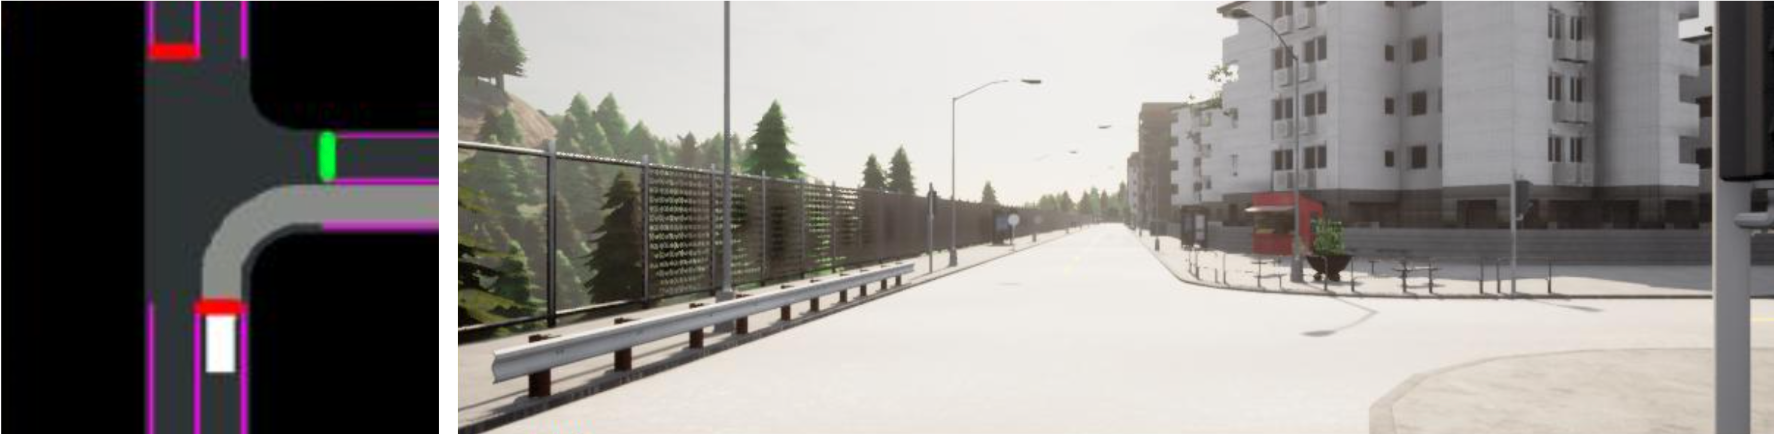
\includegraphics[width=\textwidth]{fig/TLCausalConfusionA.png}
%		\caption{Roach RL \cite{Zhang:2021}: using semantic BeV as input during training time}
%		\label{fig:TLCausualConfusionB}
%	\end{subfigure}
%	\hfill
%	\begin{subfigure}[b]{\linewidth}
%		\centering
%		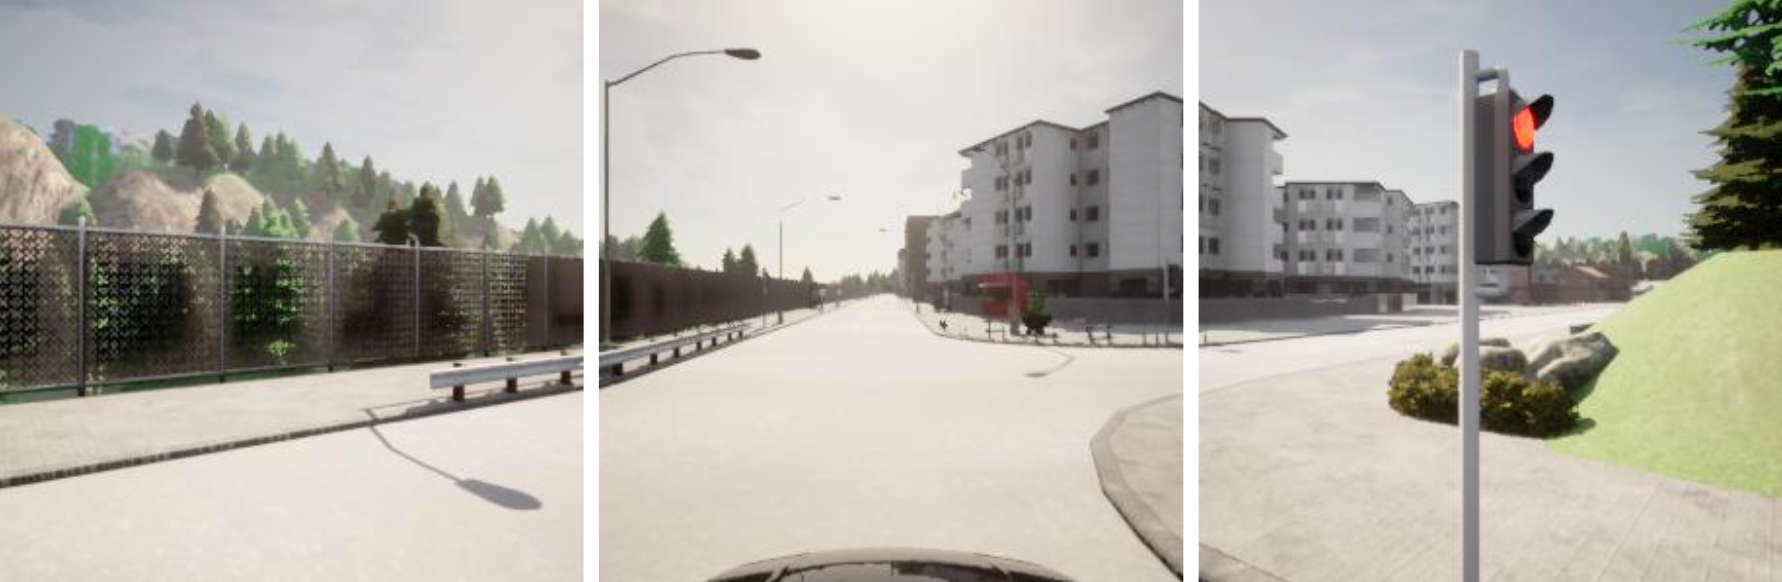
\includegraphics[width=\textwidth]{fig/TLCausalConfusionB.png}
%		\caption{BID: only images from three views as input}
%		\label{fig:TLCausualConfusionA}
%	\end{subfigure}
%	%   \includegraphics[width=1.0\linewidth]{images/TLcausalConfusion.png}
%	\caption{Top Left: The expert we use for data collection is the teacher agent Roach RL \cite{Zhang:2021}, which has access to semantic BeVs. 
%		Note that, in simulation, this expert plays the role of a human driver in the real world, who would drive to collect on-board data. 
%		Top Right: Using an insufficient FOV, the red traffic light is not observable in the image when the expert stops close to it, which may cause causal confusion when applying imitation learning to train the student agent RIM. 
%		Bottom: BID avoids this causal confusion by using a larger HFOV based on three complementary images (from different cameras). More specifically, RIM uses HFOV=$100^{\circ}$, while BID uses HFOV=$180^{\circ}$.}
%	\label{fig:causalconfusion}
%\end{figure}


\subsubsection{Multi-town Generalization}\label{sec:multi_towns_result}
\hspace{1pc}In this section, we assess the performance of BID in much more complex scenarios, as provided by CARLA's multiple towns. 
As mentioned in Sec.~\ref{sec:Dataset}, for a fair comparison, we align the training and testing settings with MILE~\cite{Hu:2022}, using CARLA's offline Leaderboard metrics (Sec.~\ref{lb_metrics}).
The results for all models trained on multi-town data are shown in Table~\ref{tab:T5_results}. 
RIM shows the worst performance among the three models, incurring more infractions, thus obtaining a significantly lower Avg.DS. 
BID achieves 98\% Avg.RC, which is on par with MILE. 
In terms of Avg.DS, MILE remains the best scoring, yielding a 73\% while BID achieves a 68\%. 
We observe that this is because MILE seldom drives outside the pre-planned lane, given the route map as input. 
On the contrary, BID lacks the explicit use of this route map since it only receives high-level navigation commands. 


% 速度、目标?
%\subsubsection{Ablation Study}
%\label{sec:Ablation Study}
%To inspect the impact of some components of CIL++, we provide an ablation study. 
%Specifically, we are interested in the fusions of input data and multi-view. 
%
%\paragraph{Input Data Fusion}
%EtE-AD models require not only sensor data but also signal information, like the ego-vehicle speed and a high-level navigation command. 
%It is interesting to study how to properly fuse these inputs. 
%To compare, we implement several types of input data fusion in Table~\ref{tab:ablation_study_inputfusion}: adding, concatenation, and tokenization. 
%In the first, the speed and command features are simply added to the image features. 
%This addition could be done either before (the default operation in CIL++) or after the Transformer Encoder block. 
%We name the latter as late fusion adding (LF.A). 
%Another common data fusion method is concatenation, which firstly stacks all the features and takes an extra join FC layer to fuse them, which we term as late fusion concatenation (LF.C). 
%Since the transformer model uses a self-attention mechanism to fuse features between tokens, we can tokenize the speed and navigation command features and feed them into the transformer block along with the image features. 
%We term this approach as Token. 
%Our results suggest that there is no obvious difference between tokenization and early adding fusion. 
%These two approaches show better results than the late fusion.
%
%
%\paragraph{Multi-view Fusion}
%CIL++ uses attention layers to fuse multi-view information. 
%To understand their contribution, we remove the transformer block and simply use the ResNet34 which retains the average pooling and an FC layer for embedding each image view. 
%The embedding outputs are then stacked and fed to the FC join layers for fusion. 
%We term this approach as view stacking (VS) in Table~\ref{tab:ablation_study_sa}. 
%The speed and command features are added to the joint embedding before feeding into the action prediction MLP. 
%We see that without the self-attention layers, the SR drops from 88\% to 70\%. 
%We think this is because the average pooling layer causes a loss of spatial information, while this information is very important for actual driving. 
%The agent should take different actions according to the location of dynamic obstacles. 
%We also use a transformer block to process the output of the ResNet average pooling layer (GAP), instead of using the flattened feature map from the last convolutional layer of ResNet34. 
%The results drop significantly, {\eg}, and the SR goes from 88\% to 64\%.


% 训练之后(多个过程)的误差曲线
%\begin{figure}[t]
%	\begin{center}
%		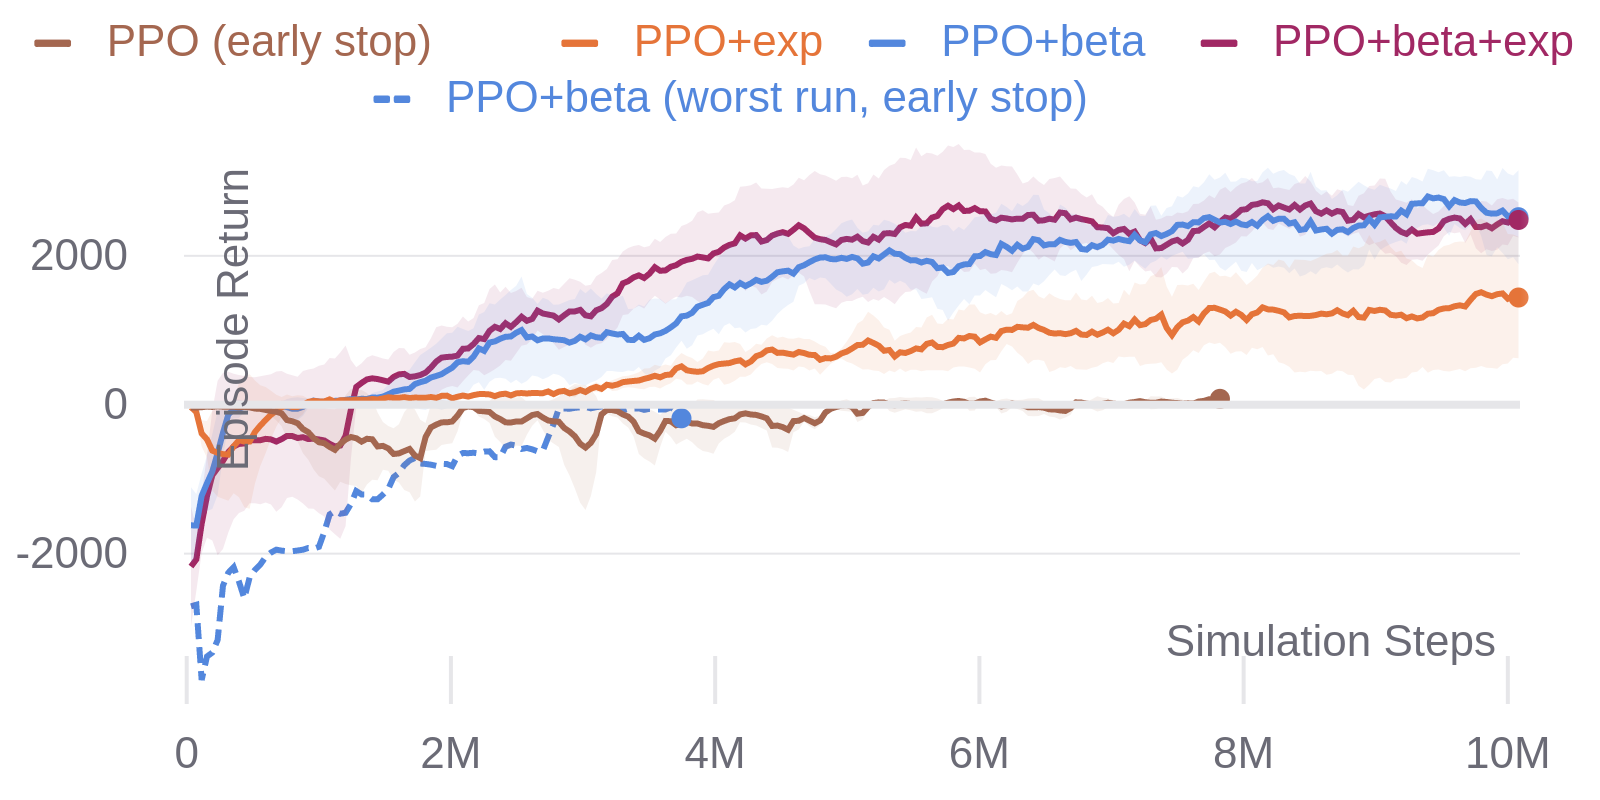
\includegraphics[width=\linewidth]{img/rl.png}
%	\end{center}
%	\vspace{-4ex}
%	\caption{\textbf{Learning curves of RL experts }
%		trained in CARLA Town 1-6.
%		Solid lines show the mean and shaded areas show the standard deviation of episode returns across 5 seeds.
%		The dashed line shows an outlier run that collapsed.}
%	\vspace{-2ex}
%	\label{fig:rl}
%\end{figure}


%\subsection{Performance of Experts}

%\textbf{\textsf{Sample Efficiency:}}
%To improve the sample efficiency of PPO, we propose to use BEV instead of camera images, Beta instead of Gaussian distributions, and the exploration loss in addition to the entropy loss.
%Since the benefit of using a BEV representation is obvious, here we only ablate the Beta distribution and the exploration loss.
%As shown in Fig.~\ref{fig:rl}, the baseline PPO with Gaussian distribution and entropy loss is trapped in a local minimum where staying still is the most rewarding strategy.
%Leveraging the exploration loss, PPO+exp can be successfully trained despite relatively high variance and low sample efficiency.
%The Beta distribution helps substantially, but without the exploration loss the training still collapsed in some cases due to insufficient exploration (cf. dashed blue line in Fig.~\ref{fig:rl}).
%Our Roach (PPO+beta+exp) uses both Beta distribution and exploration loss to ensure stable and sample efficient training.
%The training takes around 1.7M steps in each of the six CARLA servers, this accounts for 10M steps in total, which takes roughly a week on an AWS EC2 g4dn.4xlarge or 4 days on a 2080 Ti machine with 12 cores.



%\subsubsection{Driving Performance}
%
%Table~\ref{table:expert_performance} compares different experts on the NoCrash-dense and on all 76 LeaderBoard routes under dynamic weather with busy traffic.
%Our Autopilot is a strong baseline expert that achieves a higher success rate than the Autopilot used in LBC and DA-RB.
%We evaluate three RL experts - 
%(1) Roach, the proposed RL coach using Beta distribution and exploration prior.
%(2) PPO+beta, the RL coach trained without using the exploration prior. 
%(3) PPO+exp, the RL coach trained without using the Beta distribution.
%In general, our RL experts achieve comparable success rates and higher driving scores than Autopilots because RL experts handle traffic lights in a better way (cf. Table~\ref{table:infraction}).
%The two Autopilots often run red lights because they drive over-conservatively and wait too long at the junction, thus missing the green light.
%Among RL experts, PPO+beta and Roach, the two RL experts using a Beta distribution, achieve the best performance, while the difference between both is not significant. PPO+exp performs slightly worse, but it still achieves better driving scores than our Autopilot. 


%\begin{table}
%	\setlength{\tabcolsep}{2.32pt}
%	\centering
%	\begin{tabular}{lccccc}
%		\toprule
%		Suc. Rate \% $\uparrow$
%		& NCd-tt & NCd-tn  & NCd-nt & NCd-nn & LB-all  \\ 
%		\cmidrule(lr){1-1}\cmidrule(lr){2-6}
%		PPO+exp & $86 \pm 6$ & $86 \pm 6$ & $79 \pm 6$ & $77 \pm 5$ & $67\pm3$  \\
%		PPO+beta & $\mathbf{95} \pm 3$ & $\mathbf{95} \pm 3$ & $83 \pm 5$ & $\mathbf{87} \pm 6$ & $72 \pm 5$  \\
%		Roach & $91 \pm 4$ & $90 \pm 7$ & $\mathbf{83} \pm 3$ & $83 \pm 3$ & $72 \pm 6$  \\
%		\cmidrule(lr){1-1}\cmidrule(lr){2-6}
%		AP (ours) & 
%		$\mathbf{95} \pm 3$ & $\mathbf{95} \pm 3$ & $83 \pm 5$ & $81 \pm 2$ & $\mathbf{75} \pm 8$ \\
%		AP-lbc \cite{chen2020learning}
%		& $86 \pm 3$ & $83 \pm 6$ & $60 \pm 3$ & $59 \pm 8$ & N/A \\
%		AP-darb \cite{prakash2020exploring}
%		& $71 \pm 4$ & $72 \pm 3$ & $41 \pm 2$ & $43 \pm 2$ & N/A \\
%		% \bottomrule
%		\toprule
%		Dri. Score \% $\uparrow$
%		& NCd-tt & NCd-tn  & NCd-nt & NCd-nn & LB-all  \\ 
%		\cmidrule(lr){1-1}\cmidrule(lr){2-6}
%		PPO+exp & $92 \pm 2$ & $92 \pm 2$ & $88 \pm 3$ & $86 \pm 1$ & $ 83\pm0$  \\
%		PPO+beta & $\mathbf{98} \pm 2$ & $\mathbf{98} \pm 2$ & $90 \pm 3$ & $\mathbf{92} \pm 2$ & $\mathbf{86} \pm 2$  \\
%		Roach & $95 \pm 2$ & $95 \pm 3$ & $\mathbf{91} \pm 3$ & $90 \pm 2$ & $85 \pm 3$  \\
%		% Roach
%		% & $93 \pm 1$ & $91 \pm 1$ & $91 \pm 4$ & $91 \pm 4$
%		% & $79 \pm 1$ \\
%		\cmidrule(lr){1-1}\cmidrule(lr){2-6}
%		AP (ours)
%		& $86 \pm 2$ & $86 \pm 2$ & $70 \pm 2$ & $70 \pm 1$
%		& $78 \pm 3$ \\
%		\bottomrule
%	\end{tabular}
%	\vspace{-1ex}
%	\caption{\textbf{Success rate and driving score of experts.} 
%	Mean and standard deviation over 5 evaluation seeds. 
%	NCd: NoCrash-dense. 
%	tt: train town \& weather. 
%	tn: train town \& new weather. 
%	nt: new town \& train weather. 
%	nn: new town \& weather. 
%	LB-all: all 76 routes of LeaderBoard with dynamic weather. 
%	AP: CARLA Autopilot. 
%	For RL experts the best checkpoint among all training seeds and runs is used.}
%	\label{table:expert_performance}
%	\vspace{-2ex}
%\end{table}



%\subsubsection{Performance of IL Agents}
%
%The performance of an IL agent is limited by the performance of the expert it is imitating.
%If the expert performs poorly, it is not sensible to compare IL agents imitating that expert.
%As shown in Table~\ref{table:expert_performance}, this issue is evident in the NoCrash new town with dense traffic, where Autopilots do not perform well. 
%To ensure a high performance upper-bound and hence a fair comparison, we conduct ablation studies (Fig.~\ref{fig:score_eu_lb_tt_tn} and Table~\ref{table:infraction}) under the busy traffic setting such that our Autopilot can achieve a driving score of 80\% and a success rate of 90\%. 
%In order to compare with the state-of-the-art, the best model from the ablation studies is still evaluated on NoCrash with dense traffic in Table~\ref{table:sucess_rate_nc_dense}.
%
%
%The input measurement vector $\mathbf{m}_\text{IL}$ is different for the NoCrash and for the LeaderBoard. 
%For NoCrash, $\mathbf{m}_\text{IL}$ is just the speed.
%For the LeaderBoard, $\mathbf{m}_\text{IL}$ contains additionally a 2D vector pointing to the next desired waypoint.
%This vector is computed from noisy GPS measurements and the desired route is specified as sparse GPS locations.
%The LeaderBoard instruction suggests that it is used to disambiguate situations where the semantics of left and right are not clear due to the complexity of the considered map.

% 不同迭代时的消融实验
% CILv2_multiview\network\models\architectures\CIL_multiview\evaluator.py
\begin{figure*}[t]
	\centering
	\includegraphics[width=0.99\textwidth]{fig/driving_scores.pdf}
	\vspace{-1ex}
	\caption{\textbf{Driving performance and training progress of BID.} 
		All BID agents are evaluated in LBCRoutes after 30 peoch.
		Top figure. Ground truth and model prediction of steers are figured with green and blue, respectively.
		Bottom figure. The errors of training progress for every 5 epoch are displayed, including MAE (mean absolute error), MAE of acceleration and steer. 
		Results are reported as the mean over 5 evaluation seeds. 
		Others are evaluated with one seed. 
		The offline Leaderboard benchmark is used here.}
	\vspace{-1.5ex}
	\label{fig:score_eu_lb_tt_tn}
\end{figure*}


% 在密集场景中的消融实验
% table:sucess_rate_nc_dense
\begin{table}
	\caption{\textbf{Success rate of camera-based end-to-end IL agents on NoCrash-dense.}
		Mean and standard deviation over 5 seeds. 
		% 数据聚合方法:DAGGER:试图在学习策略诱导的状态分布下收集专家演示
		Our models are from DAGGER iteration 5. 
		For DA-RB, + means triangular perturbations are added to the off-policy dataset, (E) means ensemble of all iterations.}
	\setlength{\tabcolsep}{6.67pt}
	\centering
	\begin{tabular}{lccccc}
		\hline
		Success Rate \% $\uparrow$
		&  NCd-tt & NCd-tn  & NCd-nt & NCd-nn  \\ 
		\hline
		% \cmidrule(lr){1-1}\cmidrule(lr){2-5}
		SAM \cite{zhao2021sam} (0.8.4) & 
		$54 \pm 3$ & $47 \pm 5$ & $29 \pm 3$ & $29 \pm 2$ \\
		LBC \cite{chen2020learning} (0.9.6) & 
		$71 \pm 5$ & $63 \pm 3$ & $51 \pm 3$ & $39 \pm 6$ \\
		LSD \cite{ohn2020learning} (0.8.4) & 
		N/A & N/A & $30 \pm 4$ & $32 \pm 3$ \\
		DA-RB\textsuperscript{+}(E) \cite{prakash2020exploring} & 
		$66 \pm 5$ & $56 \pm 1$ & $36 \pm 3$ & $35 \pm 2$ \\
		DA-RB\textsuperscript{+} \cite{prakash2020exploring} (0.8.4)  & 
		$62 \pm 1$ & $60 \pm 1$ & $34 \pm 2$ & $25 \pm 1$ \\
		Our baseline, $\mathcal{L}$ & 
		$\mathbf{88} \pm 4$ & $29 \pm 3$ & $32 \pm 11$ & $28 \pm 4$ \\
		Our improved, $\mathcal{L}_\text{D} $ & 
		$\mathbf{88} \pm 4$ & $29 \pm 3$ & $32 \pm 11$ & $28 \pm 4$ \\
		Our best, $\mathcal{L}_\text{D}+\mathcal{L}_\text{N}$ & 
		$86 \pm 5$ & $\mathbf{82} \pm 2$ & $\mathbf{78} \pm 5$ & $\mathbf{78} \pm 0$ \\
		\hline
	\end{tabular}
	\vspace{-1ex}
	\label{table:sucess_rate_nc_dense}
	\vspace{-2ex}
\end{table}

\begin{table*}
	\caption{\textbf{Driving performance and infraction analysis of BID agents on NoCrash-busy, new town \& new weather.} 
		Mean and standard deviation over 5 evaluation seeds.}
	\setlength{\tabcolsep}{7.4pt}
	\centering
	\begin{tabular}{lccccccccc} 
		\hline
		& \begin{tabular}{@{}c@{}}Success \\ rate \end{tabular} 
		& \begin{tabular}{@{}c@{}}Driving \\ score \end{tabular} 
		& \begin{tabular}{@{}c@{}}Route \\ compl. \end{tabular} 
		& \begin{tabular}{@{}c@{}}Infrac. \\ penalty \end{tabular} 
		& \begin{tabular}{@{}c@{}}Collision \\ others \end{tabular} 
		& \begin{tabular}{@{}c@{}}Collision \\ pedestrian \end{tabular} 
		& \begin{tabular}{@{}c@{}}Collision \\ vehicle \end{tabular}  
		& \begin{tabular}{@{}c@{}}Red light \\ infraction \end{tabular}  
		& \begin{tabular}{@{}c@{}}Agent \\ blocked \end{tabular}  \\
		\hline
		% \cmidrule(lr){1-1}\cmidrule(lr){2-5}\cmidrule(lr){6-10}
		iter 5
		& \%, $\uparrow$
		& \%, $\uparrow$
		& \%, $\uparrow$
		& \%, $\uparrow$
		& \#/Km, $\downarrow$
		& \#/Km, $\downarrow$
		& \#/Km, $\downarrow$
		& \#/Km, $\downarrow$
		& \#/Km, $\downarrow$
		\\
		\hline
		%\cmidrule(lr){1-1}\cmidrule(lr){2-5}\cmidrule(lr){6-10}
		$\mathcal{L}_\mathrm{D}(\text{AP})$
		& $32 \pm 5$ & $42 \pm 3$ & $61 \pm 5$ & $76 \pm 4$ 
		& $0.53 \pm 0.55$ & $\mathbf{0}\pm0$ & $0.63 \pm 0.50$ & $3.33 \pm 0.58$ & $19.4\pm 14.4$ \\
		$\mathcal{L}_\text{D}$
		& $58\pm6$ & $65\pm3$ & $85\pm2$ & $76\pm1$ 
		& $2.06\pm1.28$ & $\mathbf{0}\pm0$ & $1.37\pm1.10$ & $1.5\pm0.2$ & $2.83\pm1.46$ \\
		$\mathcal{L}_\text{N}$
		& $75\pm2$ & $78\pm0$ & $90\pm2$ & $85\pm1$ 
		& $0.51\pm0.25$ & $\mathbf{0}\pm0$ & $0.52\pm0.17$ & $0.69\pm0.06$ & $3.36\pm0.21$ \\
		$\mathcal{L}_\text{D}+\mathcal{L}_\text{N}(\text{c})$
		& $\mathbf{88} \pm 5$ & $\mathbf{89} \pm 3$ & $\mathbf{97} \pm 0$ & $\mathbf{90} \pm 3$ 
		& $\mathbf{0.07} \pm 0.04$ & $0.01 \pm 0.01$ & $\mathbf{0.22} \pm 0.07$ & $\mathbf{0.62} \pm 0.22$ & $\mathbf{0.83} \pm 0.03$ \\
		\hline
		%\cmidrule(lr){1-1}\cmidrule(lr){2-5}\cmidrule(lr){6-10}
		BID
		& $96 \pm 2$ & $96 \pm 3$ & $99 \pm 0$ & $97 \pm 2$ 
		& $0 \pm 0$ & $0.12 \pm 0.08$ & $0.03 \pm 0.06$ & $0.14 \pm 0.18$ & $0 \pm 0$ \\
		Autopilot
		& $91 \pm 1$ & $78 \pm 2$ & $97 \pm 1$ & $81 \pm 2$ 
		& $0 \pm 0$ & $0 \pm 0$ & $0.19 \pm 0.07$ & $1.92 \pm 0.22$ & $0.17 \pm 0.09$\\
		\hline
	\end{tabular}
	\vspace{-1ex}
	\vspace{-2.5ex}
	\label{table:infraction}
\end{table*}


% 可视化注意力
\subsubsection{Visualizing BID's Attention}
\label{sec:Visualization}
\hspace{1pc}We are interested in the image content to which BID pays attention. 
Following Grad-CAM \cite{Selvaraju:2017}, gradients flow from the action space to the final convolutional layer of the ResNet backbone. 
This should produce a map that highlights the important image areas for action prediction. 
However, since BID solves a regression task, its output could be either negative or positive values, while Grad-CAM is originally designed for image classification tasks which always provide positive outputs. 
To adapt Grad-CAM to our case, we cannot merely take into account the positive gradient of the feature map. 
The computation should be divided into two cases depending on the sign of the output value. 
Negative gradients are used to calculate the weights for the feature map when the acceleration or steering angle value is lower than zero, otherwise, the positive gradient is used.


% _results\_results\CILv2\CILv2_3cam_single_lane\Eval\Valid_gradCAM_Roach_LBCRoutes_3cam_valid\30\-1\85.jpg
Fig.~\ref{fig:attention_ped_greed} shows the activation map at an intersection. 
Three image areas are highly activated: the traffic light in the right image, the crossing pedestrians in the central one, and the lane shoulder in the left one. 
Thus, we believe that BID shows a proper understanding of this scene, and a clear causality between observation and action since it decides to brake due to the pedestrians, even though the traffic light is in green and a \emph{turn-left} navigation command is given.


% 验证集的1350帧,激活图的第45张
\begin{figure}[ht!]
	\centering
	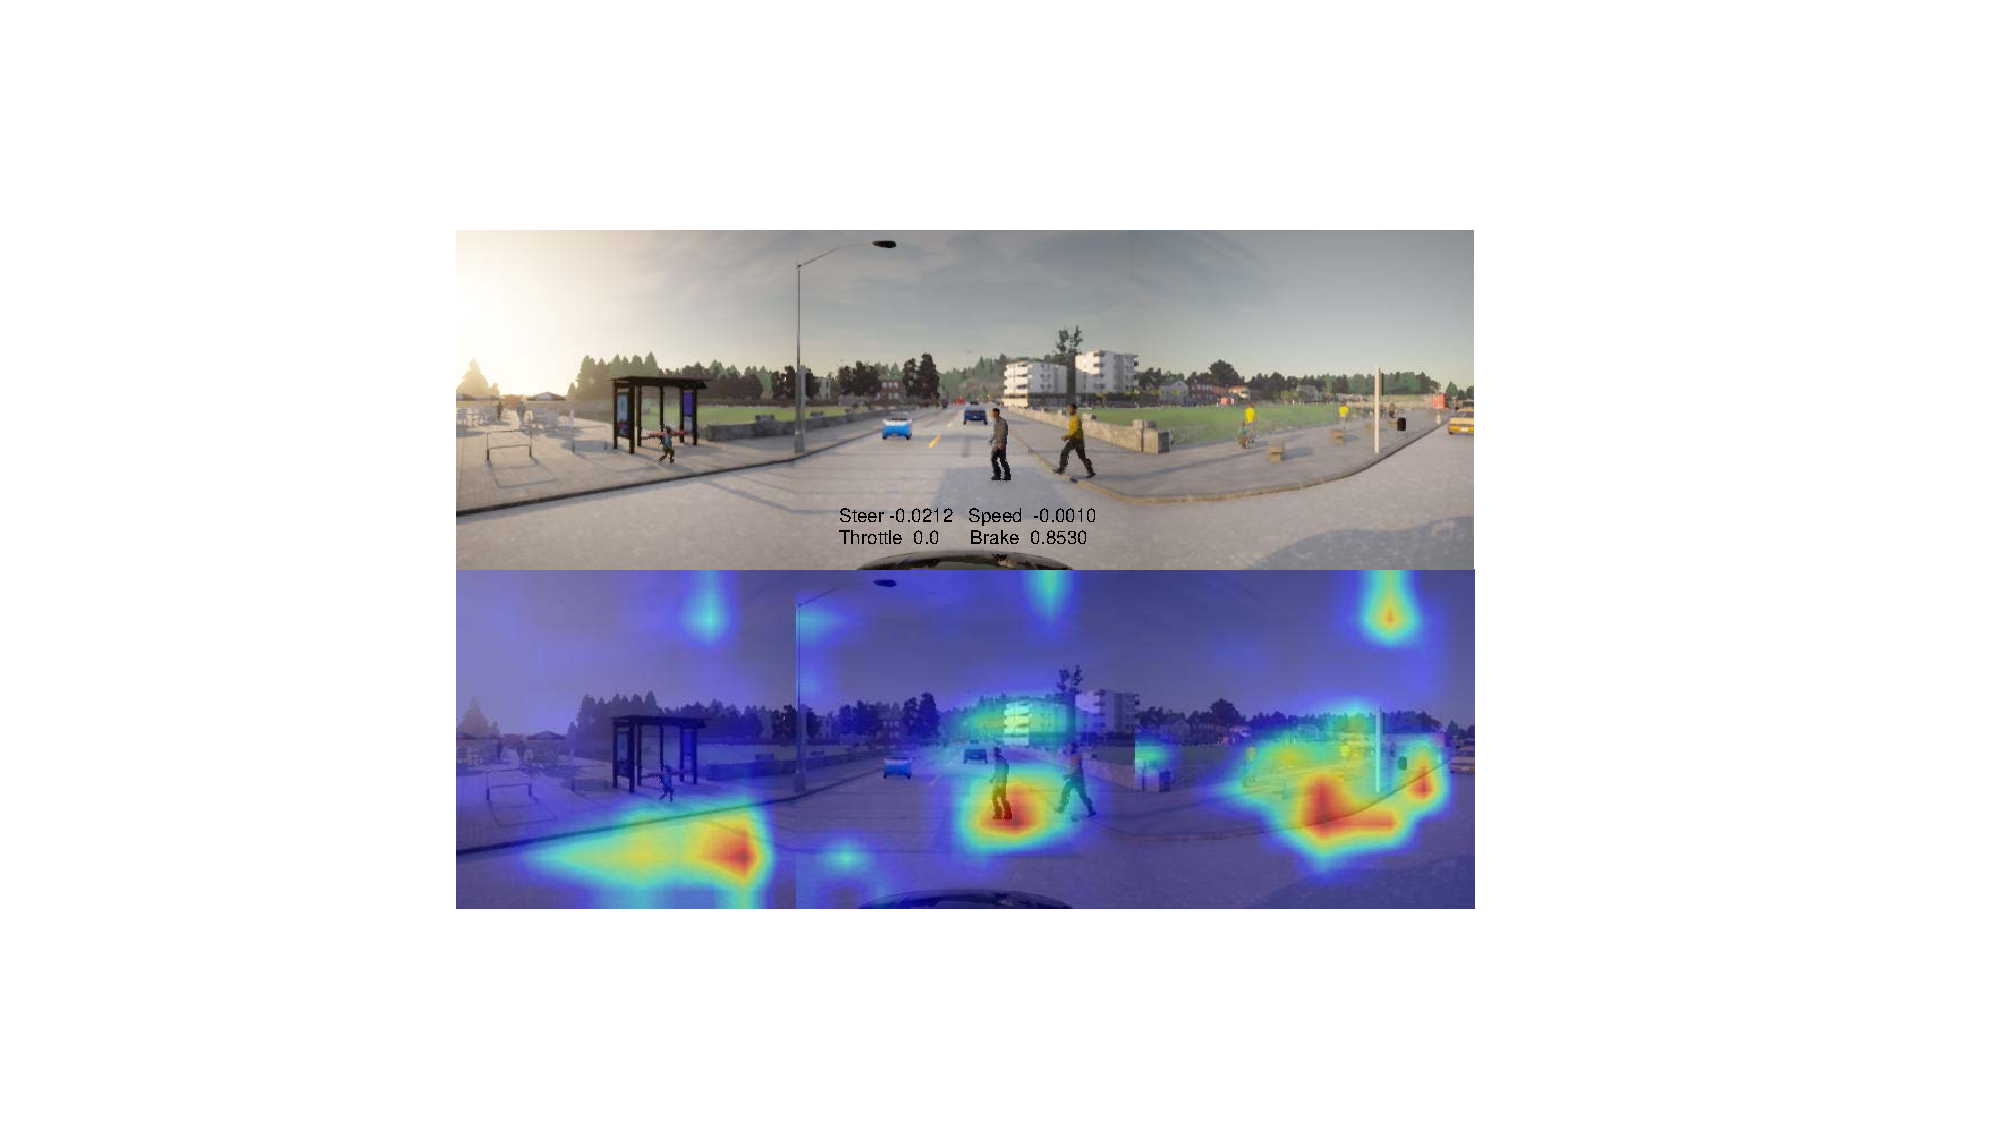
\includegraphics[width=\linewidth]{fig/attention_ped_greed.pdf}
	\caption{Activation maps of BID at an intersection in Town02. 
		Three image areas from different views are highly activated: 
		the traffic light at the right image, the crossing pedestrians at the central one, and the lane shoulder at the left one. 
		Causality between observation and action is shown as a strong braking (0.794) due to the pedestrians, even though the traffic light in green and the \emph{turn-left} command.}
	\label{fig:attention_ped_greed}
\end{figure}



% 消融实验:速度(包括背侧通路)、导航
\subsubsection{Ablation}

\hspace{1pc}The performance of an IL agent is limited by the performance of the expert it is imitating.
If the expert performs poorly, it is not sensible to compare IL agents imitating that expert.
This issue is evident in the NoCrash new town with dense traffic, where Autopilots do not perform well. 
To ensure a high performance upper-bound and hence a fair comparison, we conduct ablation studies (Fig.~\ref{fig:score_eu_lb_tt_tn} and Table~\ref{table:infraction}) under the busy traffic setting such that our Autopilot can achieve a driving score of 80\% and a success rate of 90\%. 
In order to compare with the state-of-the-art, the best model from the ablation studies is still evaluated on NoCrash with dense traffic in Table~\ref{table:sucess_rate_nc_dense}.


% 说明消融的各个指标?
The input measurement vector $\mathbf{m}_\text{IL}$ is different for the NoCrash and for the LeaderBoard. 
For NoCrash, $\mathbf{m}_\text{IL}$ is just the speed.
For the LeaderBoard, $\mathbf{m}_\text{IL}$ contains additionally a 2D vector pointing to the next desired waypoint.
This vector is computed from noisy GPS measurements and the desired route is specified as sparse GPS locations.
The LeaderBoard instruction suggests that it is used to disambiguate situations where the semantics of left and right are not clear due to the complexity of the considered map.


% 另外的
Fig.~\ref{fig:score_eu_lb_tt_tn} shows driving scores of experts and IL agents at each DAGGER iteration on NoCrash and offline LeaderBoard with busy traffic.
The baseline $\mathcal{L}$ is our implementation of baseline BID trained by expert. 
Given our improved and best BID, it is expected that $\mathcal{L}_\text{D}$ and $\mathcal{L}_\text{D} + \mathcal{L}_\text{N}$ can achieve higher success rates than those reported in Table~\ref{table:sucess_rate_nc_dense}.
The large performance gap between baseline and $\mathcal{L}_\text{D} + \mathcal{L}_\text{N}$, especially while generalizing to a new town and new weather, indicates the limitation of this baseline.


% 一步步添加后的效果
By adding dorsal stream and speed embedding based on baseline, $\mathcal{L}_\text{D}$ performs better overall than $\mathcal{L}$.
Further learning from the action distribution, $\mathcal{L}_\text{D}$ generalizes better than $\mathcal{L}$ on the NoCrash but not on the offline LeaderBoard.
Feature matching only helps when $E_s$ is provided with the necessary information needed to produce driving action.
In our case, $E_N$ contains navigational information as the desired route is provoded by nagivation command.
For the LeaderBoard, navigational information is partially encoded in $E_N$, which includes the vector to the next desired waypoint, so better performance is observed by using $E_N$.
%But for NoCrash this information is missing as $\mathbf{m}_\text{IL}$ is just the speed, hence it is impractical for $\mathbf{j}_\text{IL}$ to mimic $\mathbf{j}_\text{RL}$ and this causes the inferior performance of $\mathcal{L}_\text{K}+\mathcal{L}_\text{F}$ and $\mathcal{L}_\text{K}+\mathcal{L}_\text{F}+\mathcal{L}_\text{V}$.
To confirm this hypothesis, we evaluate a single-branch network architecture where the measurement vector $E_N$ is augmented by the command encoded as a one-hot vector.
Using feature matching with this architecture, $\mathcal{L}_\text{D} + \mathcal{L}_\text{N}$ achieves the best driving score among IL agents in the NoCrash new town \& weather generalization test, even outperforming the Autopilot.


Using value supervision in addition to feature matching helps the DAGGER process to converge faster as shown by $\mathcal{L}_\text{D} + \mathcal{L}_\text{N}$.
However, without feature matching, using value supervision alone $\mathcal{L}_\text{D}$ does not demonstrate superior performance.
This indicates a potential synergy between feature matching and value estimation.
Intuitively, the latent feature of Roach encodes the information needed for value estimation, hence mimicking this feature should help to predict the value,
while value estimation could help to regularize feature matching.


%\subsubsection{Comparison with the State-of-the-art}
%
%\hspace{1pc}In Table~\ref{table:sucess_rate_nc_dense} we compare the baseline $\mathcal{L}_\text{A}(\text{AP})$ and our best performing agent $\mathcal{L}_\text{K}+\mathcal{L}_\text{F}(\text{c})$ with the state-of-the-art on the NoCrash-dense benchmark.
%Our $\mathcal{L}_\text{A}(\text{AP})$ performs comparably to DA-RB\textsuperscript{+} except when generalizing to the new weather, where there is an incorrect rendering of after-rain puddles on CARLA 0.9.13.
%This issue does not affect our best method $\mathcal{L}_\text{K}+\mathcal{L}_\text{F}(\text{c})$ due to the stronger supervision of Roach. 
%By mimicking the weather-agnostic Roach, the performance of our IL agent drops by less than $10\%$ while generalizing to the new town and weather.
%Hence if the Autopilot is considered the performance upper-bound, it is fair to claim our approach saturates the NoCrash benchmark.
%However, as shown in Fig.~\ref{fig:score_eu_lb_tt_tn}, there is still space for improvement on NoCrash compared to Roach and the performance gap on the offline LeaderBoard highlights the importance of this new benchmark.


\subsubsection{Performance and Infraction Analysis}

\hspace{1pc}Table~\ref{table:infraction} provides the detailed performance and infraction analysis on the NoCrash benchmark with busy traffic in the new town \& weather setting.
Most notably, the extremely high ``Agent blocked'' of our baseline $\mathcal{L}_\text{A}(\text{AP})$ is due to reflections from after-rain puddles.
This problem is largely alleviated by imitating Roach, which drives more naturally, and $\mathcal{L}_\text{D}$ shows an absolute improvement of $23\%$ in terms of driving score.
In other words this is the gain achieved by using a better expert, but the same imitation learning approach. 
Further using the improved supervision from soft targets and latent features results in our best model $\mathcal{L}_\text{D}+\mathcal{L}_\text{N}$, which demonstrates another $22\%$ absolute improvement.
By handling red lights in a better way, this agent achieves $88\%$, an expert-level driving score, using a single camera image as input.



 
\section{Conclusion}
\label{sec:conclusion}
\hspace{1pc}The authors gratefully acknowledge the financial support provided by the Natural Science Foundation of Hunan Province (No.2024JJ6190), the Open Project of Xiangjiang Laboratory (No.23XJ03009), Xiangjiang Laboratory major program subproject (No.22XJ01001-2), the "Digital Intelligence +" interdisciplinary research project of Hunan University Of Technology and Business (No.2023SZJ19), Scientific research project of Hunan Provincial Department of Education (No.22B0646).
{
    \small
    \bibliographystyle{ieeenat_fullname}
    \bibliography{main}
}

% WARNING: do not forget to delete the supplementary pages from your submission 
% \clearpage
\setcounter{page}{1}
\maketitlesupplementary


\section{Rationale}
\label{sec:rationale}
% 
Having the supplementary compiled together with the main paper means that:
% 
\begin{itemize}
\item The supplementary can back-reference sections of the main paper, for example, we can refer to \cref{sec:intro};
\item The main paper can forward reference sub-sections within the supplementary explicitly (e.g. referring to a particular experiment); 
\item When submitted to arXiv, the supplementary will already included at the end of the paper.
\end{itemize}
% 
To split the supplementary pages from the main paper, you can use \href{https://support.apple.com/en-ca/guide/preview/prvw11793/mac#:~:text=Delete%20a%20page%20from%20a,or%20choose%20Edit%20%3E%20Delete).}{Preview (on macOS)}, \href{https://www.adobe.com/acrobat/how-to/delete-pages-from-pdf.html#:~:text=Choose%20%E2%80%9CTools%E2%80%9D%20%3E%20%E2%80%9COrganize,or%20pages%20from%20the%20file.}{Adobe Acrobat} (on all OSs), as well as \href{https://superuser.com/questions/517986/is-it-possible-to-delete-some-pages-of-a-pdf-document}{command line tools}.

\end{document}
